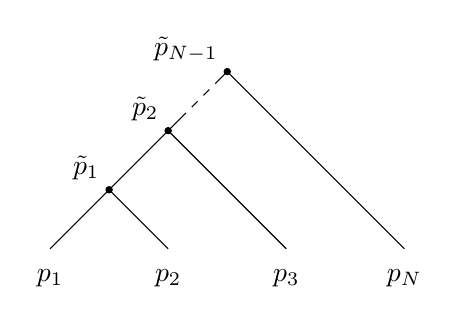
\begin{tikzpicture}[scale=1.5]
  \draw (0,0) -- (1.1,1.1);
  \draw[dashed] (1.1,1.1) -- (1.4,1.4);
  \draw (1.4,1.4) -- (1.5,1.5);
  \draw (0.5,0.5) -- (1,0);
  \draw (1,1) -- (2,0);
  \draw (1.5,1.5) -- (3,0);

  \filldraw[black] (0.5,0.5) circle (0.75pt) node[anchor=south east]{$\tilde{p}_{1}$};
  \filldraw[black] (1,1) circle (0.75pt) node[anchor=south east]{$\tilde{p}_{2}$};
  \filldraw[black] (1.5,1.5) circle (0.75pt) node[anchor=south east]{$\tilde{p}_{N-1}$};

  \draw[black] (0,-0.25) node{$p_1$};
  \draw[black] (1,-0.25) node{$p_2$};
  \draw[black] (2,-0.25) node{$p_3$};
  \draw[black] (3,-0.25) node{$p_{N}$};
\end{tikzpicture}


%%% Local Variables:
%%% mode: latex
%%% TeX-master: "main"
%%% End:
